\section{Network Topologies}\label{sec:network_topologies}
\textcolor{blue}{The title needs to be improved!\\Explain what we are trying to do once more and how our net achieves that.}\\
\textcolor{red}{Need to introduce the optimizer we are using. Probably should do so in the beginning of the evolution section.}\\
This section summarizes the results of our research, trying to find a deep learning algorithm that succeeds in detecting and classifying \gls{bns}-signals in noisy data. The goal was to not only classify the signals into the two categories ''pure noise'' and ''signal'' but also give an estimate of the signals \gls{snr}.\\
All software written for this work used the PyCBC software package \cite{pycbc} for any code involving gravitational wave data and the deep learning library Keras \cite{keras} to rapidly develop and test different network architectures. We used Tensorflow \cite{tensorflow} as the backend for Keras. \textcolor{red}{Cite specific version numbers.}

\subsection{The Data Generating Process}\label{sec:data_generating_process}
\textcolor{red}{Things missing: Mention training/validation split, mention that we shift the template around in the data (important for why we slide the generator in steps of 0.25s). ATTENTION!!! THE GENERATOR USED FOR THE TESTING SET CURRENTLY USES THE ANALYTIC PSD INSTEAD OF THE WHITEN FUNCTION! THIS IS DISPLAYED DIFFERENTLY IN THE TEXT! CORRECT EITHER THE GENERATOR OR THE TEXT! Take great care to carefully explain multirate filtering.}\\
\textcolor{blue}{Explain how the data is generated (especially that it only contains gaussian noise). Explain how training/validation set are different from the testing set used in this work. Explain how we carefully chose the parameters, especially how we got the SNR-values. Also explain the mix-and-match approach, that noise can be pure or the same noise with different signals. Also the same signal can (but this isn't necessary) have multiple noise instances. The pure noise SNR was set to 4, as that is the average value for pure noise matched filtering returns. (One might want to alter this) Finally we were careful, that no noise instance or signal from the training set is used in the validation set.}\\
Training a \gls{nn} to detect and classify \gls{bns} signals requires a large set of mock data. Using the data without some processing, however, is not possible. This is due to the fact that \gls{bns} signals are more difficult to train for than \gls{bbh} signals, as they are a lot weaker and last for a longer duration\footnote{\gls{bbh} signals spend about \SI{1}{\s} within the sensitive frequency range of our detectors, whereas \gls{bns} signals can be visible in the whitened detector data for multiple tens of seconds \cite{gw170817} and when generated even last multiple hundred seconds.}. Training a \gls{nn} on data of such duration sampled at a frequency high enough to resolve the final cycles of the binary system is not feasible, as the required network would need too many trainable parameters. However, to retain most of the \gls{snr} in the data, it is not possible to crop it to only contain a small portion of the waveform. To overcome this issue note that even though \gls{bns} signals spend a long time in the sensitive region of the detectors, their frequency evolves rather slowly and starts at low values.\\
For the early inspiral phase of the signal, frequencies are around \SIrange{30}{100}{\hertz}. To resolve these frequencies, a sample rate of \SIrange{60}{200}{\hertz} is necessary. The higher sample rates are only required for the final few seconds. For these reasons we propose to represent the data using a new multi-rate approach. Using this method, the network does not receive the data at a fixed sample rate, but rather multiple inputs, each sampling parts of the signal at different rates.\\
We choose the largest window to encompass \SI{64}{\s} of data, where a signal is aligned such, that the high frequency cutoff is roughly \SI{0.5}{\s} from the end. Afterwards we chop the data into parts of duration \SI[parse-numbers=false]{2^i}{\s} and re-sample each of these parts to have a sample rate of \SI[parse-numbers=false]{2^{12-i}}{\hertz}, with $i=0,\dotsc ,6$. This way each sample rate contains exactly $4096$ samples.\\
The 7 re-sampled data segments, however, have overlaps. This is due to the fact, that the lower sample rates contain the data of the higher sample rates, e.g. the \SI{2}{\s} interval sampled at \SI{2048}{\hertz} also includes the \SI{1}{\s} interval sampled at \SI{4096}{\hertz}. For this reason and to reduce the number of input samples even further, we only use the first $2048$ samples for each rate, except the highest one. To keep things simple however, the highest sample rate is split into two parts, each containing $2048$ samples. Therefore each \SI{64}{\s} input interval is split and re-sampled to yield 8 inputs, each containing $2048$ samples. \textcolor{red}{(Include graphic visualizing multi-rate-filtering)}
\medskip\\
To obtain a large set of training data, fake data is generated by utilizing the PyCBC software package \cite{pycbc}. \textcolor{red}{Check which version I'm using and cite that one.} The final training set contained $56250$ different signals and $161250$ different noise realizations. All waveforms were generated using the approximant ''TaylorF2'', as implemented by PyCBC. \textcolor{red}{(Should this be Lal?)} Out of the 17 parameters that could have been varied, we chose to fix the spins to be $0$ and neglected tidal effects for simplicity. Furthermore the coalescence time $t_\text{coal}$ is set to be $0$. The remaining $8$ parameters were chosen to represent a realistic distribution, in order to estimate the potential of our approach in a real search. As such, both component masses $m_1$ and $m_2$ are uniformly distributed in the range \SIrange{1.2}{1.6}{M_\odot}. Specifically we do not explicitly require $m_1\geq m_2$ when generating the waveform. The coalescence phase $\Phi_0$  and the polarization angle $\psi$ are uniformly distributed on the interval $\left[0, 2\pi\right]$ and the inclination $\iota$ is distributed like $\arccos\lr{\text{uniform}\lr{-1, 1}}$. Finally the sky-position is isotropic, i.e. $\theta$ is distributed like $\arccos\lr{\text{uniform}\lr{-1, 1}}$ and $\varphi$ uniform in $\left[-\pi, \pi\right]$.\\
The luminsoity distance $r$ is not chosen directly, but indirectly by fixing the \gls{snr} to some value. This is valid, as the \gls{snr} scales inversely with the distance. \textcolor{red}{(Is this true, or is for instance $SNR\approx 1/r^2$?))} In this work, the \gls{snr} is uniformly distributed on the interval $\left[8,15\right]$. One has to avoid one major pitfall when fixing or calculating the \gls{snr} and comparing it to other results. If one compares the \gls{snr} of two signals with the same parameters, the value will heavily depend on the length of the segment used. According to \textcolor{red}{Reference to matched filtering section}, cutting off the waveform early might result in a lower or at least inaccurate value of the \gls{snr}. For this reason, to make meaningful statements about the \gls{snr} of a signal, we need to specify how we calculated it. For this work, we generate the waveforms with a lower frequency cutoff of \SI{20}{\hertz}, which results in waveforms, with a duration of about \SI{500}{\s}. After these waveforms are generated, we calculate the projection onto the detectors and crop the signals in such a way, that they span \SI{96}{\s} and the merger lies within the last second. Only after the waveforms are cropped, we calculate the \gls{snr} with no noise present (while assuming the \gls{psd} of the detector) using the waveform itself. Since we are using multiple detectors, this value $\rho_i$ is calculated for each detector. The total \gls{snr} in the absence of noise is given by
\begin{equation}
\rho_\text{total} = \sqrt{\sum_i\rho_i^2}.
\end{equation}
Each waveform is than rescaled by multiplying with the factor $\text{\gls{snr}} / \rho_\text{total}$. As a last step, before re-sampling the data as described above, the waveforms are whitened. For the training and validation set this whitening procedure is done using the analytic \gls{psd} \verb|aLIGOZeroDetHighPower| provided by PyCBC, instead of using an estimate of the \gls{psd} based on the data itself. The testing set however uses the estimate of the \gls{psd}, and not the analytic form. The reason to treat these two sets differently from the testing set, is the way, the samples are fed to the network. For the training/validation set, we store the noise samples and pure signals separately and only add them as a first step of the network. For this reason, an estimate of the \gls{psd} would be meaningless at least for the pure signals. For the testing set however we want to mimic, how a pipeline of a detector might work. For this scenario using an analytic model would not be accurate. Therefore in this step the \gls{psd} is only estimated.\\
The reason for storing noise and signals separately are resource constraints. To cover the entire parameter-space densely enough and avoid overfitting, a large number of samples are necessary. Initially we generated and stored the sum of signal and noise, instead of storing each category separately. This has multiple disadvantages, but also one key advantage; we can use the pure signal as a filter for the optimal filter \textcolor{red}{(Insert equation number here)} and give a best-case recovery \gls{snr}, that a search could return. In that sense, we could monitor the performance and compare it to matched filtering directly during training. The disadvantages however at some point outweighed this advantage. The core disadvantage was the restricted number of samples. A file containing $500,000$ samples has a file-size on the order of \SI{200}{\giga\byte}. To train the networks on the data, we completely load it into system memory and need some overhead for formatting. To reduce these costs, we decided to split the signal- and noise-samples and only at runtime choose one instance of each category, which are than added together on the first layer of the network. The second advantage of this approach is less obvious. It enables us to easily feed the network the same signal submerged in multiple different noise realizations, which resulted in performance improvements for similar tasks (Christoph Dreißigacker, personal communication, June 2019).\\
The split between training and validation set is treated with great care, assuring, that not a single noise or signal sample from the training set is used during validation. Therefore the reported loss and accuracy values are representative of a real search. Though they are not the final statistic, we report, they are tightly linked to those and give clues about the network and its efficiency.\\
The data used for training and validating the final network contained $75,000$ different \gls{gw}-signals and $215,000$ noise realizations. We than generate a set number of unique index pairs $(s_i, n_i)$, where $s_i$ corresponds to a signal and $n_i$ to a noise sample. For the training set these indices may be selected from $s_i\in\left[0, 3/4s_t\right)$ and $n_i\in\left[0, 3/4n_t\right)$, where $s_t$ and $n_t$ are the total number of signals and noise samples respectively. If $3/4s_t\notin\mathcal{N}$ or $3/4n_t\notin\mathcal{N}$, the upper index is rounded to the nearest natural number. The total number of pairs generated is equal to the number of usable noise samples $3/4 n_t$. These index pairs represent all samples of the training/validation set that contain a \gls{gw}. In order to also supply pure noise samples to the learning algorithm, all noise realizations are also used during training. This is achieved by appending all index pairs $\lr{-1, 0}, \lr{-1, 1}, \dotsc, \lr{-1, 3/4n_t}$ to the list of index pairs generated before. Afterwards this list is shuffled. The \gls{nn} finally is fed with these $2\cdot 3/4 n_t$ samples through a function\footnote{Keras calls this function a generator.} that interprets the indices and reshapes the data.\\
The shape of the data depends on the network in use. Our final network expects a list of $16$ arrays, where each array is of shape $\lr{\text{mini-batch size, 2048, 2}}$. The last axis is the number of detectors used, whereas the second axis is the time series strain data. We generate the data for the two \gls{ligo} detectors Hanford and Livingston. \textcolor{red}{(Cite papers about these detectors. Is LIGO introduced as abbreviation?)}\\
At this point we stress again, that we use only simulated data. As such all noise that is used follows an analytic \gls{psd} \textcolor{red}{(Maybe cite the paper that gives the PSD, otherwise mention again how the PSD is called in PyCBC?)} and is gaussian. Hence no rigorous statements on the real world performance can be made.\medskip\\
To still report meaningful results, we took care of separating the data generating process for training/validation and testing set. These two sets use two different pipelines to generate the data. The testing data is supplied as continuous time series data, cut into large chunks. This chunk is than handed to a function\footnote{Again, this is a generator in Keras terms.} that takes \SI{64}{\s}

\subsection{Evolution of the Architecture}\label{sec:evolution_of_architecture}
\textcolor{blue}{Talk about the different things we tried, what didn't work and how we improved on them. (Improvement from convolution to inception, improvement from inception to collect-inception, improvement from inception to tcn-inception, improvement of tcn-collect-inception over collect-inception.)}\\
\textcolor{red}{Talk about the different loss functions used for the two outputs. Also mention their loss weights and training algorithms? Talk about general points we found, i.e. using dropout makes loss a little less stable but improves performance even when a lot of samples are used. (compare (24.06.2019) and (25.06.2019 (1)), (19.06.2019) and (25.06.2019 (2))) Decreasing learning rate in Adam did not help (19.06.2019).}\\
This section gives an overview of the steps that were taken to arrive at the final architecture. It will chronologically highlight the pivotal points along the way and showcase some ideas that did not work out. A detailed timeline can be found in \cite{network_wiki}. \textcolor{red}{(Should the wiki be turned into a PDF and migrated to github?)}\\
As a starting point we tried to use an easy case, where the \gls{snr} was uniformly distributed between 10 and 50, with all other parameters fixed. The neutron stars were modeled with $m_1=m_2=$ \SI{1.4}{M_\odot}. The data was stored and loaded as the sum of signal and noise and contained data for the two detectors Hanford and Livingston. In general, the data contained samples of signals and pure noise realizations. Until stated otherwise, all of the following networks use this data.\\
To rate the performance of a network we didn't use the sensitivity of the network yet. Instead we used the variance and mean squared error of the recovered \gls{snr}-values compared to the label values in order to estimate performance. The hope was that these simple statistics correlate strongly with the actual sensitivity.\medskip\\
The first architecture we used was very close in nature to that of \cite{huerta_parameter_estimation}, halving, however, the number of filters in each convolution layer and using batch normalization in between the convolution and activation. Therefore, we used a network of 3 stacked convolution layers, each followed by a batch normalization, ReLU activation \textcolor{red}{(Never introduced the ReLU activation)} and maximum pooling layer. The number of filters was doubled after each convolution layer. Since the input data to our network is sampled at multiple rates, this network has 14 input channels instead of 2. (7 input channels per detector, where each of the 7 channels corresponds to a single sample rate)\\
Though initially trained without pure noise samples and with only the \gls{snr} as training goal, we soon changed to use the data as mentioned in the beginning of this section. Furthermore, we added a second output. This second output gives a number between 0 and 1, where 1 corresponds to the network classifying the data as signal and 0 for classifying it as pure noise. If the output is neither 0 nor 1 one can use a threshold to determine if the output should correspond to a signal or pure noise. By default the threshold value is set to $0.5$. We will refer to the results this output gives as ''p-value'' throughout this work, even though it is not really a probability. As this second output tries to categorize the results into two different classes, we cannot use mean squared error as a loss for this output. Instead we use a loss called categorical crossentropy, which is designed to optimize classification problems. As we are using two different losses now, the network will optimize the sum of the mean squared error from the \gls{snr}-output and the categorical crossentropy from the p-value output. This furthermore requires us to split the last layer into two.\\
All of the following analysis is based purly on (13.02.2019) in \cite{network_wiki} and its limited information. Therefore, a lot of the statements below are only qualitative rather than quantitative.\\
The network was able to recover the \gls{snr} of signals rather well but has a large spread for the recovered \gls{snr} values of pure noise samples. The sensitivity can be eyeballed to reach 100\% only above \gls{snr} $\sim 25$ and dropping close to 0\% below \gls{snr} $\sim 20$. The latter is caused by the high \gls{snr} values assigned to certain noise samples, some reaching values of up to $\sim 20$. Furthermore, evaluating the second output on 3000 signals from the validation set gives an accuracy of about 95\% and a false positive rate of about 6\%. These numbers don't sound terrible but are in context. First of all, signals are expected to be in the \gls{snr}-range of 5-15 \textcolor{red}{[Citation]}. At these values the false positive rate seems to be a lot higher than the 6\% over the entire validation set. Secondly, a false positive rate of 6\% equates to a false alarm rate of about \SI[per-mode=fraction]{6e5}{\samples\per\month}\footnote{This crude calculation uses 0.5 as a threshold value. Therefore, one gets $6\times 10^5$ samples with the output being larger than 0.5 per month.}. Ideally the false alarm rate should not exceed \SI[per-mode=fraction]{10}{\samples\per\month} above an \gls{snr} of about $8$. A month for this work is defined to be \SI{30}{\days}.\medskip\\
From this point the first major iteration was the introduction of inception modules \cite{inception_module}. They replaced the simple convolution layers of the architecture used previously(see 15.02.2019 and 03.04.2019 in \cite{network_wiki}). Furthermore, guided by \cite{inception_module}, the inception modules were preceeded by 2 convolution layers. The implementation of the inception module was as a first step a direct adaptation of the original work \cite{inception_module}. It used kernel sizes of $\lr{1,3,5}$. With these kernel sizes results did not improve but rather got worse. Increasing the filter sizes to $\lr{4,8,16}$, however, proved to be a useful change. The performance in mean squared error, variance and false positive rate improved significantly, with the false positive rate reaching $\sim 0.015\%$. By eye, the sensitivity also made an improvement as the loudest false positive was estimated to have \gls{snr} $\sim 15$. With this, the sensitive went up to 100\% around \gls{snr} 20 and only dropped to 0\% below \gls{snr} $\sim 12$. Though this is still not an impressive performance, it is a considerable improvement over the simple convolution approach.\medskip\\
Having found the new inception architecture, we conducted a test to figure out which of the 7 sample rates benefit the network the most. To view the full results see 04.04.2019 and 05.04.2019 of \cite{network_wiki}. We found, that each sample rate, except for the \SI{64}{\hertz} one, benefits the results. Using only the sample rates (\SI{2048}{\hertz}, \SI{512}{\hertz}, \SI{128}{\hertz}) gave comparable results to using the channels (\SI{2048}{\hertz}, \SI{1024}{\hertz}, \SI{512}{\hertz}, \SI{256}{\hertz}, \SI{128}{\hertz}). Furthermore, shallower networks seemed to yield similar or improved performance, when compared to deeper ones. Shallower and deeper in this case refers to the number of stacked inception modules.\medskip\\
Having found that using only the sample rates (\SI{2048}{\hertz}, \SI{512}{\hertz}, \SI{128}{\hertz}) is at least a good approximation to using all sample rates, we tested a new architecture. Previously all sample rates were fed to the network in terms of channels of the same convolution layer. The new architecture assigned a stack of inception modules for each sample rate. This way the channels only represent the different detectors. The result of each stack are than concatenated and fed to some final layers. In the beginning the stacks for different sample rates had different depth. We found however that the network functioned best when each stack had the same depth. Furthermore, results improved when the stacks were not too deep. We settled on an architecture that had a depth of 3 inception modules in each stack, deployed another 2 inception modules after concatenation and condensed them down to the ouput size by the use of 2 dense layers per output.\\
As a last step, we tested the performance of using the three sample rates mentioned above against using all sample rates. Here using all sample rates improved the results significantly. Therefore, the performance quoted below is derived from the network using all sample rates. For the full history on the evolution and architecture of these kinds of network see (12.04.2019 (2)) through (17.04.2019) in \cite{network_wiki}. From here on out, we will call a network that uses individual stacks of layers for each sample rate a collection network. Therefore we call the kind of network described above a ''collect-inception network''.\\
The final iteration of this architecture broke the previous records of mean squared error and variance against the label values. With a false positive rate of $\sim 0.3\%$, it did perform worse than the previous record holder. This was, however, not the metric we judged the performance by at that point in time. Therefore, this network was thought of as the best one. By eye, one can also estimate that the sensitivity didn't drop to 0\% even at \gls{snr} 10 and reaching 100\% at \gls{snr} $\sim 18$. In this aspect the network improved.\medskip\\
The performance of this newest iteration of the network was good enough for us to move on to a more difficult data set. For this one we only changed the \gls{snr} range. Instead of varying it between 10 and 50, we went down to varying it between 8 and 15. Furthermore, we introduced sensitivity and false alarm rate as new metrics to gauge performance. We calculate both of these statistics for each of the two outputs and in the following way.\\
The false alarm rate is a measure that tells us how many outputs above a given value are to be expected in a month of data, when the network evaluates it. To estimate this function we need to sample
\begin{equation}\label{def:false_alarm_rate}
f(x)=\text{number of noise samples estimated louder than }x\text{ per month}.
\end{equation}
To explain how we estimate this function, we will talk only about \gls{snr}. The process for the p-value, however, is equivalent.\\
The values for $x$ we can sample are the predictions of the network over all pure noise samples. We will denote the number of pure noise samples by $m$. Each of these noise samples $n_i$ is evaluated by the network and assigned a \gls{snr} value of $x_i$. To estimate $f_i\coloneqq f(x_i)$, we define $f_i'\coloneqq \left|\left\{ x_j > x_i | j\in \left[1, m\right]\right\}\right|$. $f_i'$ therefore is a number of samples. To convert it to samples per month, we calculate the observation time, i.e. the time the total number of samples $m$ corresponds to. To do so, we observe that for each signal the waveform is allowed to move around in the noise background by \SI{\pm 0.25}{\s}. Therefore, when we evaluate a continuous time series, we need to shift the network across the data with a step-size of \SI{0.25}{\s}. With this the observation time the $m$ samples cover is $m\cdot\vphantom{0.25}$\SI{0.25}{\s}. Therefore, $\frac{f_i'}{m\cdot 0.25}$ is in units ''samples per second''. From this we find $f_i=\frac{f_i'}{m\cdot 0.25}\cdot2,592,000$\SI[per-mode=fraction]{}{\samples\per\month} as an estimate for $f$. We usually plot these results in a semi-log-scale plot, as the false alarm rate drops exponentially when going to higher \gls{snr}s.\\
To explain the sensitivity, we will again only go into detail about how we do this in terms of \gls{snr}, as the process for the p-value is equivalent.\\
The sensitivity is a measure of how large the percentage of samples in a certain \gls{snr} bin are that get assigned a value larger than some threshold. We choose this threshold as the largest value that was attributed to some noise sample in our validation set, as we want to keep false alarms as low as possible. Therefore the first thing we do is find this maximal value. In a second step we look at all samples from the validation set, that contain a signal. For each of these signals the \gls{snr} value was chosen when injecting it into noise. For this reason, we can bin the samples based on this known value. Therefore, the x-values are the \gls{snr} values. (This is true also for the p-value case.)\\
The corresponding y-value is the number of samples in a bin assigned a higher value than our threshold over the total number of samples in a bin. In the case that a bin is empty, we assign it the value 0.\\
For the first few iterations the sensitivity is calculated slightly wrong, as the p-value output was used in the case of the \gls{snr}-sensitivity to judge whether or not we were looking at a false positive. As the outputs for \gls{snr} and p-value, however, seems highly correlated, the difference this made is not significant and most of the plots are close to the real sensitivities. The false alarm rates were also not calculated correctly for the first few plots, as they were always scaled by the same factor, regardless of how many samples the validation set actually contained.\medskip\\
After using the previously best known architecture and taking a quick look at the sensitivity it was able to reach, we were inspired by \cite{tcn_idea} to try a new kind of network, called temporal convolutional network (\gls{tcn}). Their results suggested, that a stack of dilated convolution layers outperforms normal convolution layers. Their idea was backed up by findings of \cite{tcn_paper}, who showed that \gls{tcn} are better suited for sequence data than other architectures. We could however not directly test their implementation as they did not reveal their entire architecture. \textcolor{red}{(I don't have access to the quoted paper in its present state, so maybe they did reveal it. Can I get access?)}\\
As we are training for \gls{snr} and p-value, one immediate problem of a pure \gls{tcn} would be the output shape. This kind of network was originally designed to generate and alter sequence data and thus returns a tensor of the same length per channel as its input had. This would be great, if we could generate a \gls{snr} time series for all inputs. It is, however, not trivial to do so and for our purposes impractical\footnote{Defining a \gls{snr} time series for a time series that is sampled at multiple rates is the technical difficulty. The impracticality does only come in, when we store noise and signal separately, as we would need to generate the \gls{snr} time series on the fly, which is computationally rather expensive.}. The first intuitive solution to the problem of reshaping would simply be to use dense layers to scale down the output to the desired dimensions. We did try this approach rather late (see (25.07.2019 (1)) in \cite{network_wiki}) but it was without success. Instead, we tried to use the \gls{tcn} as a denoising stage in front of every input stack of the collect-inception-network. To do so, we fed each input to a \gls{tcn} and added an auxiliary output afterwards. This output used a mean squared error loss to fit the pure waveform in the Livingston detector. The output of the \gls{tcn} is than added back onto the input and fed into a stack of 3 inception modules. The result of each such stack are finally concatenated and fed into dense layers. Each \gls{tcn} consisted of 12 diluted convolution layers. The number of convolution layers was chosen such that the receptive field of the \gls{tcn} covers the entire length of the input, i.e. 4096 samples. The idea behind adding the \gls{tcn}-output back onto the input was to amplify signals, whilst not throwing away information, if the \gls{tcn} was not able to recover a signal. Details of this architecture and the results we found can be viewed at (03.06.2019) in \cite{network_wiki}. \textcolor{red}{(Insert image of general architecture)}\\
Using the \gls{tcn} as a denoiser required us to change the way the samples are fed to the network, as we needed the pure \gls{gw}-signal for the training goal. Thus, instead of feeding the network the sum of signal and noise, it receives the two parts separately and adds them together on the first layer. When evaluating real samples the network will be fed the sum of signal and noise instead. This is not a problem though, as one of the two inputs can simply receive zeros as input. This is a change to the data generation we decided to keep. For a detailed reasoning as to why we decided to change to this new system see \autoref{sec:data_generating_process}.\\
The performance of this network exceeded those of any previous network by a considerable margin. Now judging by sensitivity rather than mean squared error or variance, it dropped below 80\% sensitivity only for \gls{snr}s smaller 12 and didn't considerably drop below 20\% at all. The sensitivity improved especially at low \gls{snr}s. Using $37,500$ noise samples the false alarm rate can be resolved up to about \gls{snr} 9, as that is the value of the loudest sample. Below \gls{snr} 9 the false alarm rate is rather high with a lowest value of about \SI[per-mode=fraction]{300}{\samples\per\month}. Using more noise samples would enable us to finer resolve the false alarm rate. As it is not feasible during development, to evaluate each individual network on a large set of data, we will only use the sensitivity to get a rough estimate of the performance and compare different algorithms in that regard. For the final network a large testing set will be used in order to more finely resolve the false alarm rate and to make stronger statements on the sensitivity.\\
From here on out we will refer to a network of the kind described in this part as \gls{tcn}-collect-inception network or \gls{tcin}. Though it improves almost all statistics we are using, when compared to a standard collect-inception network, it comes at a cost. This cost is the memory the network needs in order to be trained. In the form used for these results, it used up \SI{30}{\giga\byte} of video memory on a NVIDIA GV100 while already reducing the mini-batch size to 24. This graphics card is currently the only one that has enough memory to support such an architecture. The availability of this hardware is very limited and thus does not allow for rapid development. A smaller alternative would therefore be beneficial.\\
We also conducted a test, trying to determine if the \gls{tcn} is able to reconstruct the original waveform from a noisy time series. These tests showed that it is not consistently able to do so. Using mean average percentage error as a loss function and setting the noise free signal as the training goal for a pure \gls{tcn}, the loss did not fall below $70,000$. Trying to train the \gls{tcin} without the use of an auxiliary loss function, however, proved to deteriorate performance (see (24.07.2019 (2) in \cite{network_wiki} for details). So other \gls{tcin}s use the auxiliary outputs as well.\medskip\\
After the success of \gls{tcin}s, we searched for simpler architectures to reduce memory constrains. For that reason we tried using an old record holder, a simple inception network that was very memory efficient. To improve its preformance, residual connections were added to all inception layers where it was possible to do so without needing to use dimensional reduction layers. This choice was motivated by a conversation with Christoph Dreißigacker and the results of \cite{residual_connections_invention}. The residual connections are meant to help the network learn as it is more easily able to recover the identity mapping between the input of an inception module and its output (see (26.06.2019 (1)) and (27.06.2019 (1)) in \cite{network_wiki}). The total network consisted of 8 stacked inception modules with one intermediate pooling layer and 6 residual connections. Networks using mainly inception modules and combining them with residual connections will be called inception-res networks from here on out. The inception modules were preceded by two convolution layers. The different sample rates were fed to the network as different channels of the same input layer. It also only used the three sample rates (\SI{2048}{\hertz}, \SI{512}{\hertz}, \SI{128}{\hertz}). By accident, the kernel sizes in the inception modules were set to $(1,2,3)$. This did, however, prove to be beneficial to the network.\\
The results this network produced were incredible and outperformed anything we had seen so far. Sensitivities stayed close to or above 60\% for all \gls{snr} bins and the loudest noise sample was estimated at an \gls{snr} of $\sim 7.8$. One thing that seemed strange though, was the plot of recovered \gls{snr}s, when plotted against the label values. For some specific \gls{snr} values, the predictions were scattered but lower by a significant margin. This can be seen as streaks in the plots. \textcolor{red}{Insert and reference to plot here.}\smallskip\\
The observed behavior and the incredible performance was due to a bug in how the network was fed with data. The generator combines a pure waveform with one noise realization to create a signal sample and is supposed to combine an array of zeros with a noise realization for a pure noise sample. A missing ''if''-statement led to the array of zeros always being replaced with the waveform that was the last in the list of available waveforms. Therefore, instead of pure noise, the network always saw noise plus one specific waveform. The same error with the exact same waveform was present in both the training and the validation set which made this error hard to catch. In fact the error was only discovered about two weeks after it first occurred. Finding the bug this late led to the optimization of the architecture for this flawed data. The best performing network had a sensitivity of more than 95\% over the entire \gls{snr} range for this flawed data, even once we used more difficult data, i.e. varying more parameters than just the \gls{snr}.\\
Though this mistake might at first seem like a waste of time, it actually helped in two aspects. Firstly, it showed the possibility for a network to consistently recover a single sample from different noise realizations and being able to model it well enough. The hurdle for a general search isn't trivial from this point, as in an optimal case we would expect the network to generalize the structure of the waveforms it was trained on and interpolate a template bank, but it is a starting point. Secondly, the optimization led to architectures with improved performance over for instance the \gls{tcin}s, when evaluated on non-flawed data. For this reason, we will list a few of the notable improvement here.\smallskip\\
The first observation was that the mistake of using filter sizes $(1,2,3)$ was actually an improvement over using $(4,8,16)$, which was previously used and found to be beneficial (see (27.06.2019 (2)) in \cite{network_wiki}). Another feature introduced was the reduced number of input samples. Before the different sample rates had some overlap in the time domain, i.e. the last second of the data was sampled by all 7 rates, the last 2 seconds were sampled by all but the highest sample rate and so on. As the higher sample rates also contain all the information the lower sample rates do, this overlap was thrown away. For a detailed description of how this non overlapping multi-rate sampling work see \autoref{sec:data_generating_process}. A study, testing the two different approaches to sampling the data and reducing the number of input samples by simply using less sample rates, showed that using all sample rates is beneficial, while the cropping the overlapping part of the data has no negative effect. (see 02.07.2019 (2) and following in \cite{network_wiki})\\
With the performance these architectures suggested, we moved to more difficult data, altering not only the \gls{snr} but also component masses $m_1, m_2$, coalescence phase $\Phi_0$, sky-position $\theta, \varphi$ and inclination $\iota$. As expected, the performance decreased a bit using more difficult data. Trying to recover the old performance led to one of the final improvements to the architecture. Instead of using a single inception stack, we introduced an architecture that is a mixture of the collect-inception networks and the pure inception networks. It uses the same inputs as the collect-inception networks, but than cascades down, concatenating two stacks after two inception layers, reducing the initial 8 stacks to 4. These 4 stacks each are fed through two further inception layers before being concatenated again. This procedure is repeated a third time, which results in a single stack of inception layers which is than fed to dense layers, in order to get the outputs. See \autoref{fig:cascade_inception_res_net} for an overview of the architecture. We will still refer to networks with a similar structure as collect-inception-res networks.\\
It again improved results a by a little. The sensitivity now didn't drop below 97\% for any of the bins, with the loudest noise sample having an \gls{snr} $\sim 8$. This is the last and best performing iteration of the network we found before the bug in the generating process was discovered and fixed. It therefore is still one of the core structures of the final architecture.\medskip\\
\begin{figure}
\centering
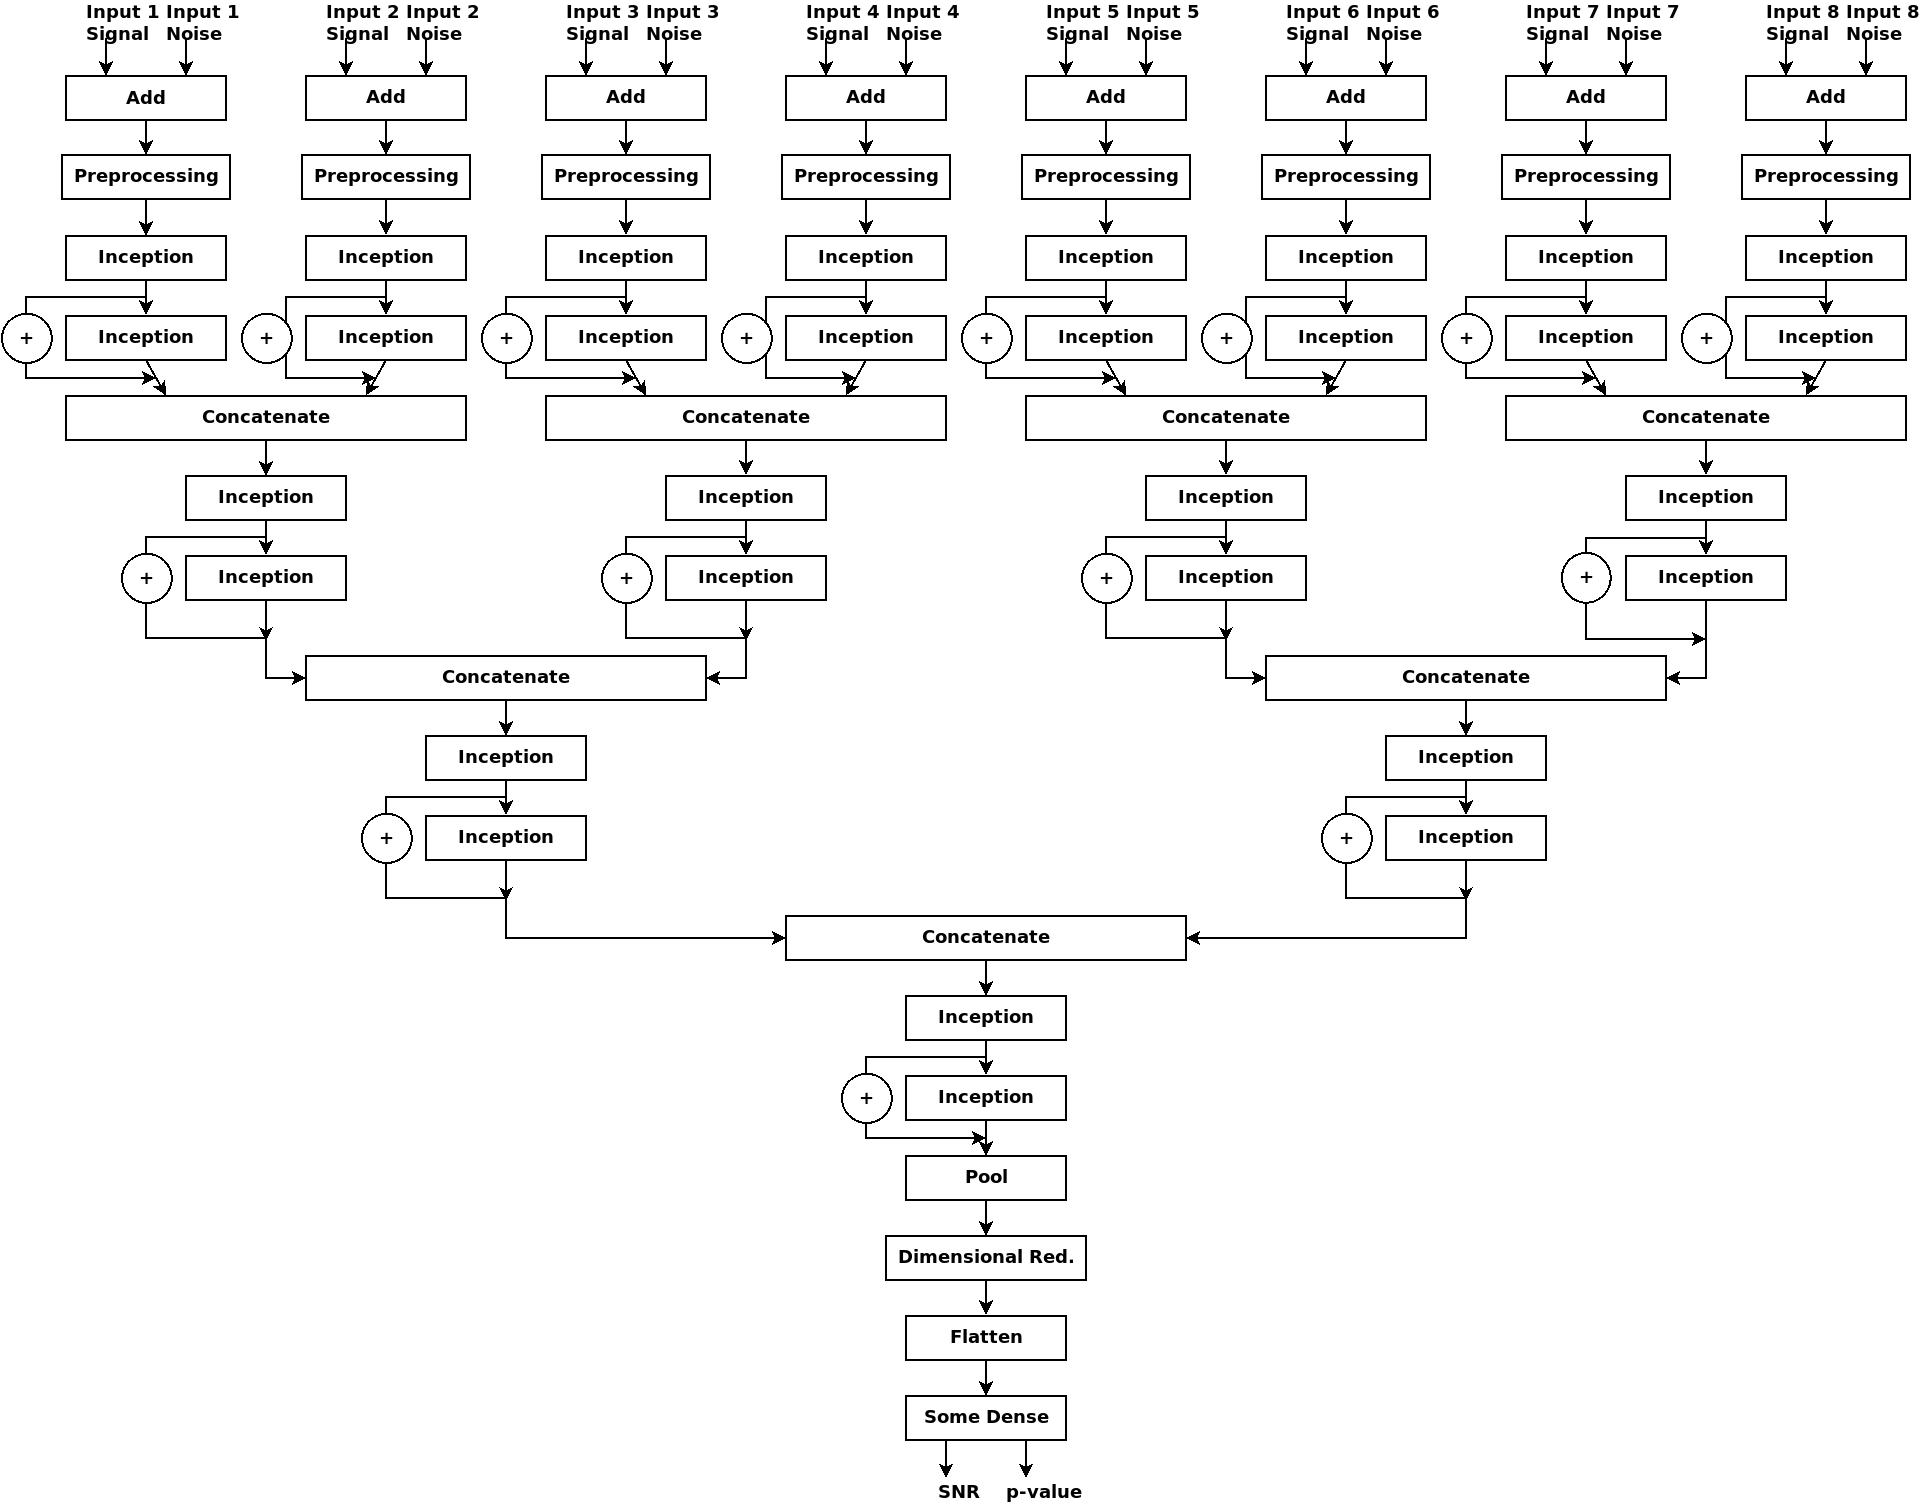
\includegraphics[width=\textwidth]{collect_inception_res_net_rev_1.png}
\caption[Cascading architecture of a collect-inception-res network]{The rough architecture of a cascading collect-inception-res network is shown. The preprocessing layers contain 2 convolution layers as well as some dropout and batch normalization. The block labeled ''Some Dense'' actually consists of two separate stacks of dense layers, that reduce the output of the last inception layer down to the appropriate size. \textcolor{red}{Work on this graphic and make it a bit larger.}}\label{fig:cascade_inception_res_net}
\end{figure}

\noindent Using the corrected data generator with the previously well performing inception-res networks on data, where all previously mentioned parameters were being varied, showed how big an impact the error made. The sensitivity dropped from 95\% in every \gls{snr} bin to below 20\% in the loudest bin. The collect-inception-res network held up a bit better, dropping to 40\% sensitivity in the loudest bin. From this point we tried to recover some of the lost performance by developing new features and implementing them into the collect-inception-res network.\medskip\\
One of the first tests was training the network to just optimize the p-value rather than both \gls{snr} and p-value. This did however not work and decreased the performance of the network significantly, reaching only $\sim 12\%$ at the loudest point. Using the original architecture and adding in one more inception module per stack resulted in worse performance overall, but not by much.\smallskip\\
One of the problems the network has is that estimating pure noise with a large \gls{snr} value significantly decreases sensitivity. An overestimated noise sample thus is a lot worse than an underestimated signal. Therefore we tried to implement a loss function that mimics this behavior, by growing exponentially for overestimating noise and only linearly for underestimating it. For signals this behavior is mirrored, i.e. the loss grows exponentially for underestimating signals and linearly for overestimating them. The details on how this loss looks like and how it was derived can be found in \autoref{app:custom_loss}. It turned out that this approach also didn't help but rather decreased the sensitivity of the network. It even seemed to push the two categories closer together (see 21.07.2019 in \cite{network_wiki}). Other tests (e.g. (22.07.2019 (2)) in \cite{network_wiki}) showed similar results.\medskip\\
Another approach we took was close in nature to that of SincNet \cite{sincnet}. SincNet convolves the input data with a parameterized filter, that is used in standard signal processing. This has two main advantages. Firstly, the filters the network applies become more interpretable and thus reveal more insight into what the network is actually trying to accomplish. Secondly, the number of trainable parameters is reduced as we don't need to train a large convolution kernel but rather some parameters of a known function. Their implementation used the parametrized layer only as the first layer of the architecture and showed improvements over other purely convolutional approaches when trying to recognize speakers \cite{sincnet_speach}. Based on this work we used our adaptation only as a first layer, too. Instead of using Sinc-functions, we tried to use sums of sine waves. The convolution kernel is thus given by $\sum_{i=1}^n A_i\cdot\sin\lr{f_i t + \varphi_i}$, where $A_i$, $f_i$ and $\varphi_i$ are learned parameters and $t$ is used to sample the function. The general idea behind this approach is to enable the network to construct a crude template of a general waveform by combining multiple sine waves. To restrict the available frequencies, the layer is given a low and high frequency cutoff. This restriction is necessary to determine the shape of the convolution kernel. To sample a sine wave of frequency $f$, according to Nyquist, one needs to sample at least with a rate of $2f$. Therefore the sample rate is given by $\diff t = \frac{1}{2 f_\text{high}}$. As we want to fit at least one complete cycle of the lowest frequency into our kernel, the number of samples in the kernel is given by $N=\frac{f_\text{low}}{2f_\text{high}}$. By default the convolution kernel will always be filled with samples, e.g. a sine wave of frequency $f=2f_\text{low}$ will manage two full cycles in the convolution kernel. We called this layer ''Wave-Convolution'' or ''WConv1D'' in short and will from here on out refer to it by this name.\\
To get a quick estimate of how well this new approach does we devised a simple network consisting of only two convolution-type layers and two dense layers to get the correct output. We than compare two iterations of this network, one trained with the new Wave-Convolution layer and one using a usual convolution layer. All other parameters are kept constant. For the convolution layer, we choose the kernel size in such a way that the number of trainable parameters is on a comparable scale.\\
First tests of this new layer did apply some false windowing and used a skewed methodology. The results produced by these early tests lost out to pure convolution quite strongly and thus this approach was not further pursued. \textcolor{red}{INPUT RESULTS OF FINAL TESTS HERE! (maybe remove the sentences before, if the results stay terrible)}\medskip\\
As no architectural alteration proved to be highly beneficial to the performance of the network for the difficult data where a lot of parameters are varied, we went back to using the data that only varies the \gls{snr}. We than combined the general approach of the \gls{tcin} with the new cascading architecture and found that it outperforms the traditional \gls{tcin}. This combination is the final architecture we tried and will be explained in further detail in \autoref{sec:final_architecture}.


\subsection{Final Network}
\textcolor{blue}{Talk about how the final network looks, how it performs and what could be imporved.}\\
\textcolor{red}{First final network stored at tcn\_collect\_inception\_res\_net\_rev\_6\_248201905643}
\subsubsection{Architecture}\label{sec:final_architecture}
\textcolor{blue}{Explain the architecture and the reasoning behind it. Talk about the size of the model, where it could be trained and what the drawbacks of the architecture are. (Drawbacks: Large memory size (hence small batch size), very deep $\to$ slow training and maybe vanishing gradients, hyper-parameter-optimization is hard, not everywhere are residual connections (fixable by further dimensional reduction))}
\subsubsection{Network Performance}\label{sec:network_performance}
\textcolor{blue}{Evaluate the performance of the network. Show sensitivity curves, talk about speed advantages, how does it in both cases compare to matched filtering? How does it compare to related works? (Reference the BNS-Net paper, what is different between our approach and theirs? Why does theirs seem to work a lot better? Does it?)}
%\textcolor{blue}{Compare the speeds of both methods, the accuracy. What kind of drawbacks does the network have, what are its advantages, how should it be used and understood? (Not as a standalone method of analysis but rather as a starting point for samplers and a quick way of estimate certain properties.)}
